\documentclass[a4paper]{scrartcl}%{{{

\usepackage{float}
\usepackage{tikz}
\usetikzlibrary{arrows,automata}
\usepackage{pgf}
\usepackage[utf8]{inputenc} % this is needed for umlauts
\usepackage[ngerman]{babel} % this is needed for umlauts
\usepackage[T1]{fontenc}    % this is needed for correct output of umlauts in pd
\usepackage{amssymb}
\usepackage{amsmath}
\usepackage{mathabx}
\usepackage{mathrsfs}
\usepackage{dsfont}
\usepackage{graphicx}
\usepackage{fancyhdr}
\usepackage{lastpage}
\usepackage{imakeidx}
\setlength{\parskip}{\medskipamount}
\setlength{\parindent}{0pt}
\usepackage{enumitem}
\usepackage{hyperref}
\usepackage{verbatim}

%%%%%%%%%%%%%%%%%%%%%%%%
% Kopf- und Fusszeilen %
%%%%%%%%%%%%%%%%%%%%%%%%
\pagestyle{fancy}
\lhead{
        Maximilian Roth
}
\chead{Logik-Tutorat Lösungen Blatt 8\\}
\rhead{
        \today{} \\
        Seite \thepage{} von \pageref{LastPage}\\
        
}
\lfoot{}
\cfoot{}
\rfoot{} 

%%%%%%%%%%%%%%%%%%%%%%%%
% Anfang des Dokuments %
%%%%%%%%%%%%%%%%%%%%%%%%%}}}

\begin{document}
\section*{Disclaimer}%{{{
\label{sec:disclaimer}
Auch in diesem Dokument können sich Fehler befinden!\\
Sie sind nicht die Musterlösung der Aufgaben, sondern selbst erstellte Lösungen.\\

Als generelle Lektüre kann ich nur das Skript von Markus Junker aus dem WS 17/18 empfehlen:\\
\url{http://home.mathematik.uni-freiburg.de/junker/skripte/InfoLogik.pdf}\\
Hier ist vieles sehr genau und verständlich erklärt.%}}}

\section*{}%{{{
\label{sec:aufgabe_1}

    \begin{figure}[H]
        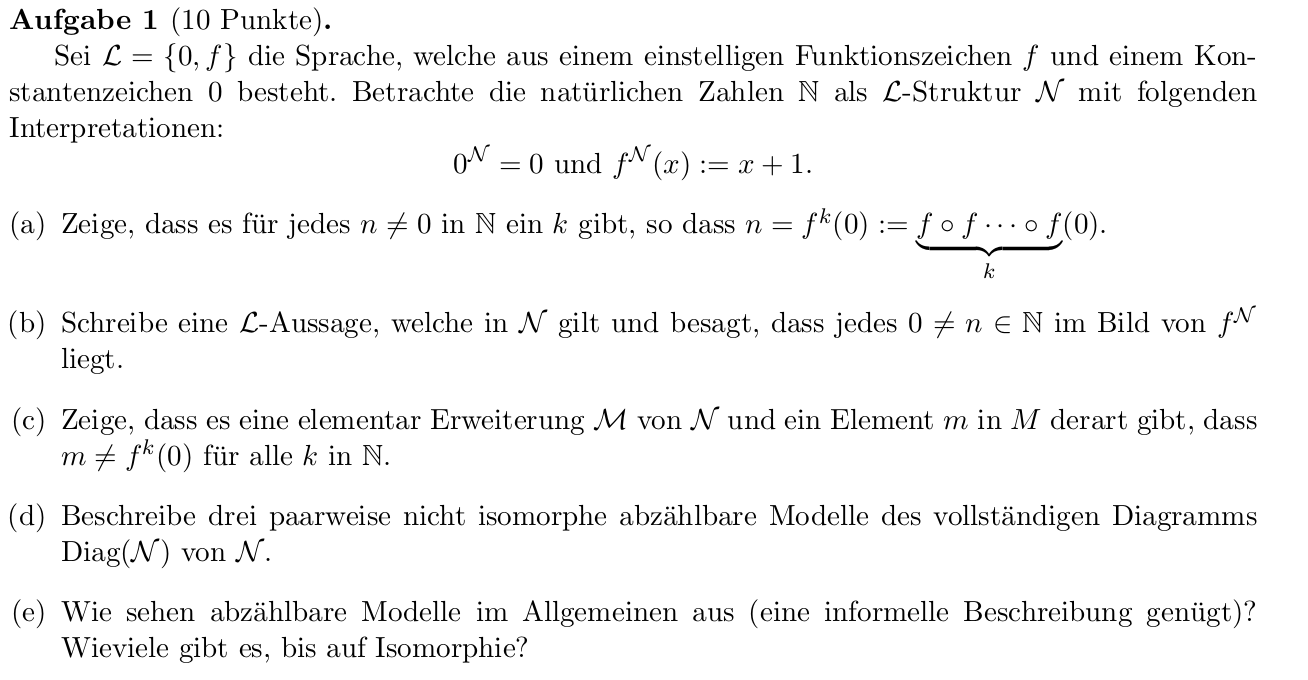
\includegraphics[scale=0.3]{./A-1.png}
        \label{fig:}
    \end{figure}

    Im folgenden steht f immer für $f^\mathcal{N}$
    \begin{itemize}
        \item a)\\
            Wir zeigen mit Induktion über n:\\
            \begin{itemize}
                \item IA: n = 1\\
                    $f^1(0) = 0 + 1 = 1$\\
                \item IV: Gelte die Beh. für ein n mit $f^k(0) = n$\\
                \item IS: $n \rightarrow n+1$:\\
                    $n + 1 = f^1(n) \overset{IV}{=} f^1(f^k(0)) = f^{k+1}(0)$\\
            \end{itemize}
        \item b)\\
            $\forall n (\neg n \doteq 0 \rightarrow \exists x(f(x) \doteq n))$\\
        \item c)\\
            Sei $\varphi_k = m \doteq f^k(0), k \in \mathds{N}\backslash\{0\}$\\
            Dann gilt mit $m \neq f^k(0), \forall k \in \mathds{N}\backslash\{0\}$ auch $\neg \varphi_k, \forall k \in \mathds{N}\backslash\{0\}$\\
            \\Wir zeigen zunächst, dass $\mathcal{M}$ existiert und dann, dass es elementare Erweiterung ist:\\
            \begin{itemize}
                \item $\mathcal{M}$ existiert:\\
                    Wir zeigen, dass $\mathcal{N}$ und $\neg \varphi_k, k \in \mathds{N}\backslash\{0\}$ sich nicht wiedersprechen,\\
                    also dass $T = Diag(\mathcal{N}) \cup \{\neg \varphi_k | k \in \mathds{N}\backslash\{0\}\}$ konsistent ist.\\
                \item $\mathcal{M}$ ist elementare Erweiterung von $\mathcal{N}$\\
            \end{itemize}
        \item d)\\
        \item e)\\
    \end{itemize}


%}}}

\newpage

\section*{}%{{{
\label{sec:aufgabe_2}

    \begin{figure}[H]
        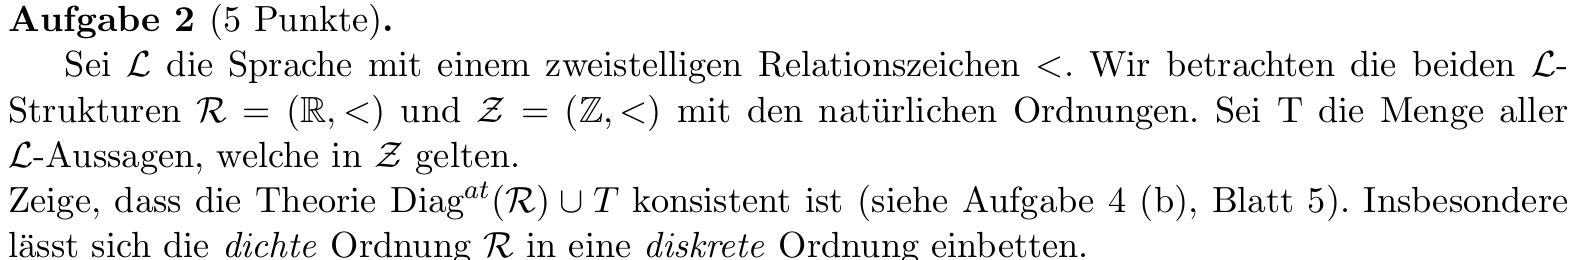
\includegraphics[scale=0.3]{./A-2.png}
        \label{fig:}
    \end{figure}

    \begin{itemize}
            Wir zeigen die Konsistenz für eine endliche Teilmenge $\Sigma \subseteq_{endlich} Diag^{at}(\mathcal{R})$,\\
            um danach den Kompaktheitssatz anzuwenden.\\
            \\Nun überlegen wir uns, welche Aussagen in $\Sigma$ sein können:\\
            Alle die, die etwas darüber aussagen, dass ein Element strikt kleiner, als ein anderes ist.\\
            \\Da $\Sigma$ endlich ist können auch nur endlich viele Elemente aus $\mathds{R}, \{r_1,\dots,r_n\}$ darin vorkommen.\\
            \\Es gilt weiter, wenn O.B.d.A. gilt: $r_1 < \dots < r_n$, dann gilt auch:\\
            \begin{center}
                \\$\underline{\bigwedge_{i=1}^{n-1} r_i < r_{i+1}} \vdash A \in \Sigma$\\
            \end{center}
            (mit dem wissen, dass < die natürliche Ordnung ist und damit ihren Regeln unterliegt)\\
            \\Um obige Formel ausdrücken zu können benötigen wir eine Sprache mit entsprechenden Konstantenzeichen: 
            $\mathcal{L}^* = \mathcal{L} \cup \{d_{r_1}, \dots, d_{r_n}\}$\\
            \\Sei also $\psi = \bigwedge_{i=1}^{n-1} r_i < r_{i+1}$, dann gilt $\psi \vDash \Sigma$\\
            \\Wenn $Z^*$ eine $L^*$-Struktur ist mit $d_{r_i}^{Z^*} = i$ ist folgt:\\
            \\$\Rightarrow Z^* \vDash \psi$ und $Z^* \vDash T$\\
            $\Rightarrow Z^* \vDash \Sigma \cup T$ \quad (und damit konsistent)\\
            $\overset{Kompakth.}{\Rightarrow} Diag^{at}(\mathcal{R}) \cup T$ konsistent\\
        \item Man kann eine dichte lineare Ordnung in eine diskrete einbetten\\
            Z ist diskret mit T, aber elementare Erweiterung von der dichten Ordnung $\mathcal{R}$\\
    \end{itemize}
%}}}

\section*{}%{{{
\label{sec:aufgabe_3}

    \begin{figure}[H]
        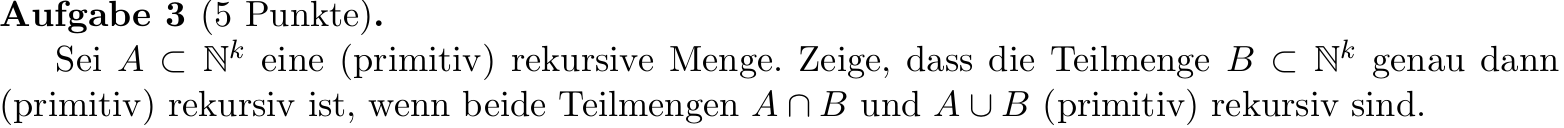
\includegraphics[scale=0.3]{./A-3.png}
        \label{fig:}
    \end{figure}

    \begin{figure}[H]
        \centering
        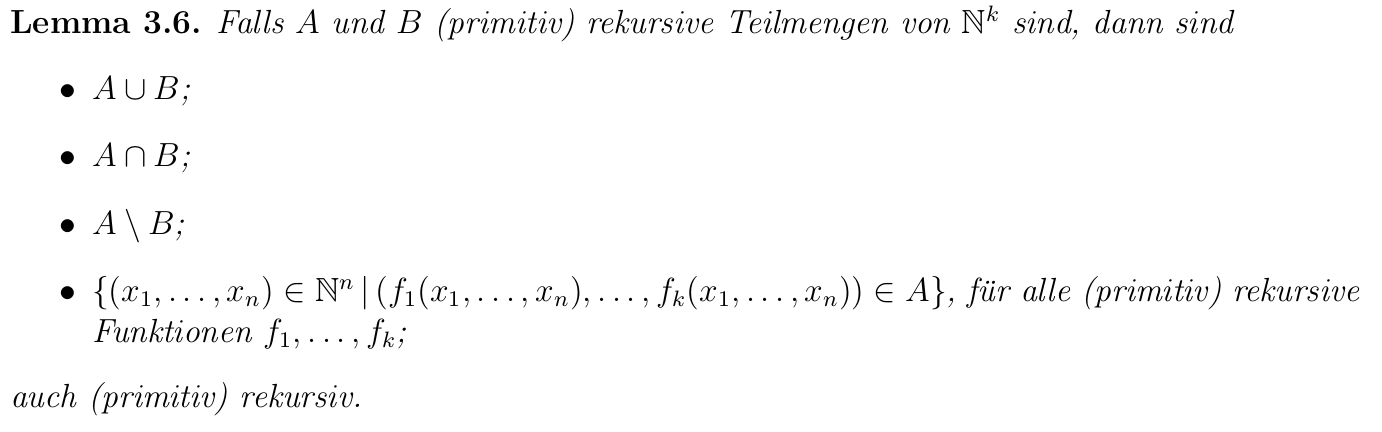
\includegraphics[scale=0.3]{./prim-rek.png}
        \label{fig:./prim-rek}
    \end{figure}

    \underline{ZZ:} B (prim.) rek. $\Leftrightarrow A, A \cup B, A \cap B$ (prim.) rek.\\
    \begin{itemize}
        \item "$\Rightarrow$":\\
            Folgt direkt mit Lemma 3.6\\
        \item "$\Leftarrow$":\\
            Es gilt $B = (A \cup B) \backslash (A \backslash (A \cap B))$ (siehe Venn-Diagramm)\\
            Weiter gilt:\\
            \begin{figure}[H]
                \centering
                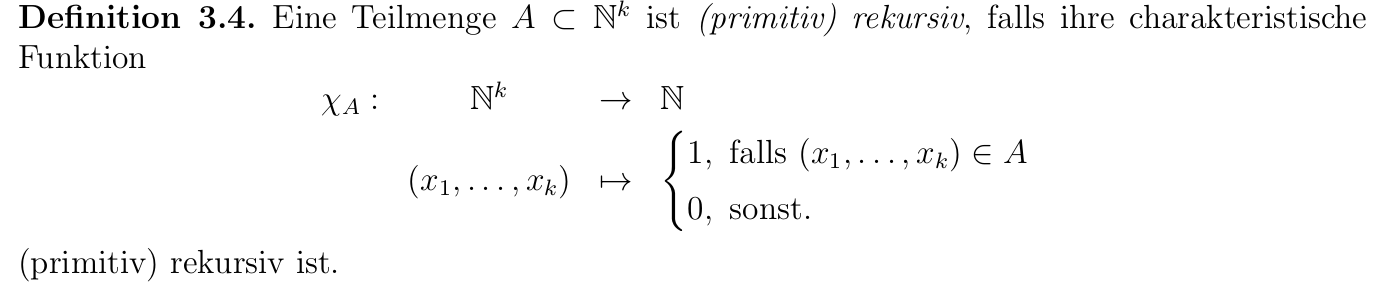
\includegraphics[scale=0.3]{./char-fkt.png}
                \label{fig:./char-fkt}
            \end{figure}
            Und X\textbackslash Y ist prim. rek., da $\chi_{X\backslash Y} = \chi_X \dotdiv \chi_Y$ prim. rek. ist. (Nach Bsp. 3.2)\\
            \begin{figure}[H]
                \centering
                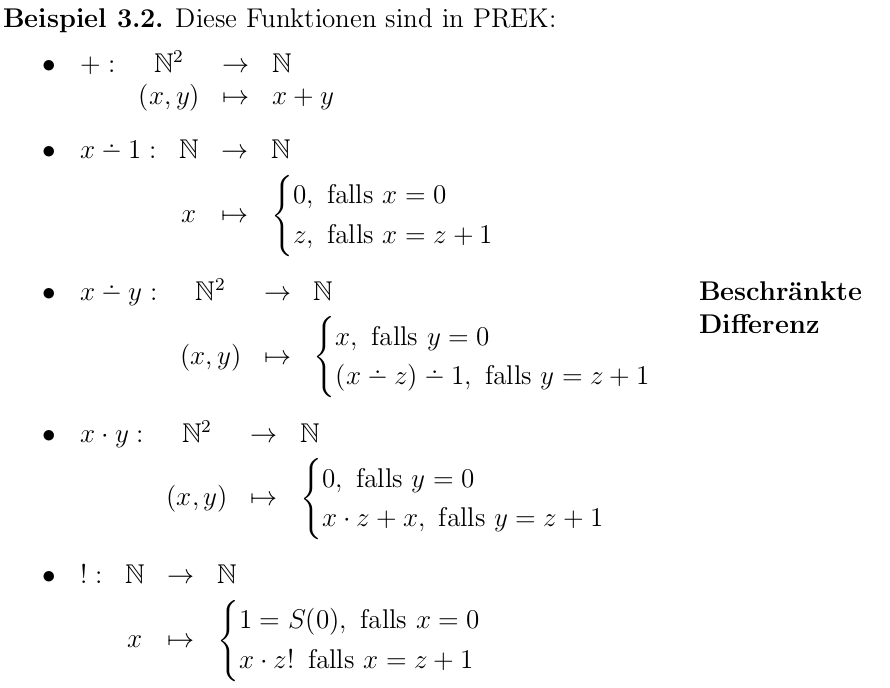
\includegraphics[scale=0.3]{./dotdiv.png}
                \label{fig:./dotdiv}
            \end{figure}
             

    \end{itemize}
    



%}}}

\end{document}
